\begin{figure}[!htbp]
\centering
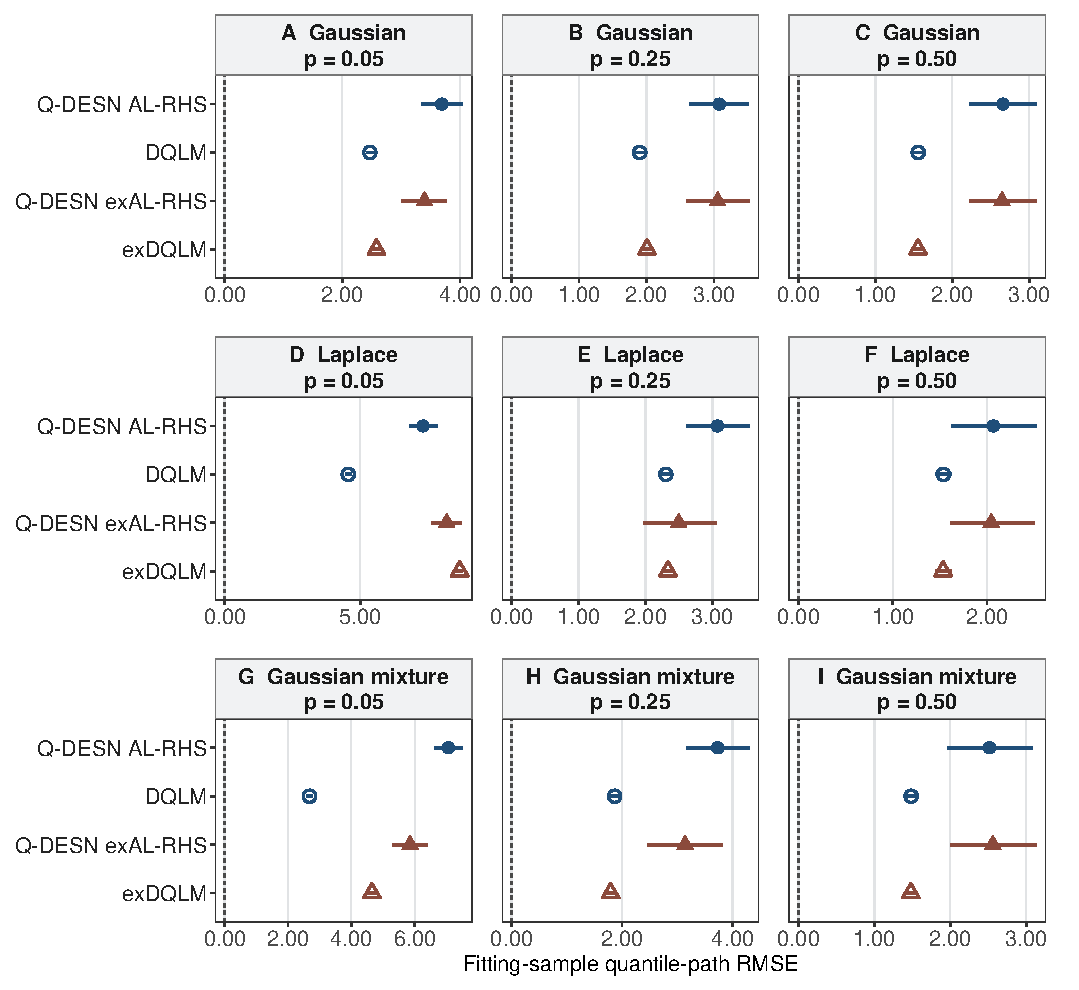
\includegraphics[width=0.98\textwidth]{figures/independent_simulation/qdesn_pro_review_vb_fit_rmse.pdf}
\caption{Variational fitting-sample recovery in the single-quantile study. Points and approximate equal-tailed 95\% intervals summarize quantile-path RMSE under the variational fit; lower values are better. Model encodings follow Figure~\ref{fig:simulation-500obs-mcmc-fit-rmse-intervals}. Panels A--I identify the observation-error family and probability level, with separate horizontal scales. The dashed line marks exact recovery. The summaries condition on the simulated series and the criterion-specific specification.}
\figalt{Nine panels compare approximate variational fitting-sample
quantile-path RMSE means and 95 percent intervals for four models across three
observation-error families and three probability levels. Lower values are better.}
\label{fig:simulation-500obs-vb-fit-rmse-intervals}
\end{figure}
